% =========================================================================
% Section 5: Joint Observation-Computation Adaptive Policy via Fast LBAP
% File: docs/paper/sections/03_adaptive_policy.tex
% =========================================================================

\section{Joint Observation-Computation Adaptive Policy via Fast LBAP}
\label{sec:adaptive_policy}

In wireless edge reception, automatic modulation classification (AMC) encounters two fundamentally distinct operational bottlenecks: (i) physical waveform observation latency $T_{\mathrm{acq}} = N / f_s$ dictated by the analog-to-digital converter (ADC) sampling rate $f_s$ and window length $N$ \cite{guo2025fewer}, and (ii) digital inference processing latency $T_{\mathrm{comp}}$ induced by arithmetic and memory operations in the host processor or dedicated tensor accelerator \cite{liu2026beacon, denboer2021fpga}. 

Existing dynamic AMC strategies treat these dimensions in isolation. On one hand, adaptive sample-length techniques (e.g., Fewer-Sample \cite{guo2025fewer}) scale $N$ using a single neural backbone, but operate under the ideal assumption of perfectly synchronized, non-dispersive AWGN channels ($\mathrm{CFO} = 0$), failing when rotational or multipath distortions require representational richness rather than raw temporal averaging. On the other hand, early-exit deep architectures (e.g., BEACON \cite{liu2026beacon}, Joint Early Exit \cite{liu2025joint}) adapt arithmetic depth across internal branches while holding the input observation window strictly static ($N = 128$), completely ignoring physical acquisition latency $N / f_s$.

To bridge this fundamental research gap, we formulate a \emph{joint observation-computation} decision framework. The proposed receiver initiates classification from a short physical prefix $N_0 = 256$ samples and dynamically selects among three heterogeneous operational actions: terminating immediately with an ultra-fast conventional classifier ($a_0$), acquiring an extended physical observation $N_1 = 512$ samples ($a_1$), or escalating computation by executing a deep multi-domain expert on the existing prefix ($a_2$). To govern this decision without oracle inputs or runtime overhead, we develop the \emph{Fast Learned Benefit-Aware Predictor} (Fast LBAP), a hybrid Ridge--MLP estimator running in under $0.05\,\mathrm{ms}$ that directly predicts net utility and distinguishes recoverable errors from structurally irrecuperable channel failures.

% -------------------------------------------------------------------------
\subsection{Tripartite Action Space and Zero-Leakage Observable Prefix}
\label{subsec:action_space}

Let $r[n]$ denote the complex baseband received signal sampled at rate $f_s$. The receiver captures an initial observation prefix $\mathbf{r}_{256} = [r[0], r[1], \dots, r[N_0-1]]^T \in \mathbb{C}^{N_0}$ of length $N_0 = 256$ samples ($32$ baud at nominal oversampling factor $\mathrm{sps} = 8$). The adaptive policy $\pi$ operates upon an observable gating vector $\mathbf{g}(\mathbf{r}_{256})$ extracted exclusively from this prefix, choosing an action $a \in \mathcal{A} = \{a_0, a_1, a_2\}$:

\begin{enumerate}
    \item \textbf{Action $a_0$ (Fast Baseline Evaluation):} The receiver extracts a standardized $65$-dimensional feature vector $\mathbf{f}_{256}$ (comprising cyclic moments, high-order cumulants $C_{20}, C_{40}, C_{42}, C_{60}, C_{63}$, spectral flatness, and envelope statistics \cite{xia2026optimal}) and classifies the transmission using a pre-trained Support Vector Machine ($\mathrm{SVM}_{256}$ with an RBF kernel). This action consumes the minimal observation horizon $N_0 = 256$ and requires low computational complexity.
    
    \item \textbf{Action $a_1$ (Extended Physical Observation):} The receiver waits for the front-end to buffer an additional $\Delta N = N_1 - N_0 = 256$ samples, forming an extended window $\mathbf{r}_{512} \in \mathbb{C}^{N_1}$ ($N_1 = 512$ samples, $64$ symbols). Features $\mathbf{f}_{512}$ are extracted and evaluated via an extended Support Vector Machine ($\mathrm{SVM}_{512}$). This action incurs an unavoidable physical acquisition latency penalty $\Delta T_{\mathrm{acq}} = \Delta N / f_s$, but reduces the empirical variance of high-order statistical cumulants ($\mathrm{Var}(\hat{C}_{42}) \propto 1/N$).
    
    \item \textbf{Action $a_2$ (High-Capacity Multi-Domain Computation):} The receiver terminates physical acquisition at $N_0 = 256$ samples ($\Delta T_{\mathrm{acq}} = 0$), routing the raw I/Q tensor to a high-capacity deep neural expert ($\mathrm{MultiDomainAMCNet}$) executed on GPU or edge accelerator cores. As established in Section~\ref{sec:architecture}, this expert simultaneously deploys an in-GPU RRC matched-filter front-end, a $16$-channel 1D ResNet with Squeeze-and-Excitation, a $6$-channel multi-harmonic spectral branch, a $25$-channel polyphase symbol Transformer, and a $120$-dimensional statistical residual MLP. This action expands representational capacity to resolve phase ambiguity, residual CFO, and multipath interference without awaiting additional physical symbols.
\end{enumerate}

\begin{figure}[t]
\centering
\resizebox{\columnwidth}{!}{%
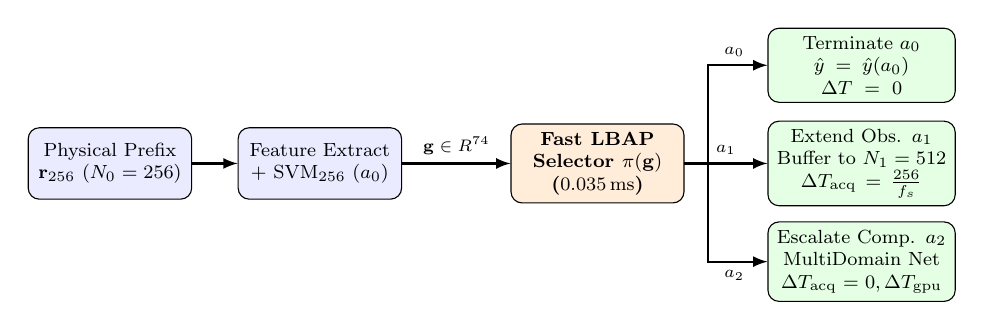
\begin{tikzpicture}[scale=0.86, every node/.style={transform shape}]
    % Styles
    \tikzset{
        block/.style={rectangle, draw, fill=blue!8, text width=6.2em, text centered, rounded corners, minimum height=3.0em, font=\footnotesize},
        gate/.style={rectangle, draw, fill=orange!15, text width=6.6em, text centered, rounded corners, minimum height=3.2em, font=\footnotesize\bfseries},
        action/.style={rectangle, draw, fill=green!10, text width=7.2em, text centered, rounded corners, minimum height=3.0em, font=\footnotesize},
        line/.style={draw, -latex, thick}
    }

    % Nodes with wide explicit coordinates to prevent arrow/label collisions
    \node [block] (input) at (0, 0) {Physical Prefix\\$\mathbf{r}_{256}$ ($N_0=256$)};
    \node [block] (base) at (3.1, 0) {Feature Extract\\+ $\mathrm{SVM}_{256}$ ($a_0$)};
    \node [gate] (lbap) at (7.2, 0) {Fast LBAP\\Selector $\pi(\mathbf{g})$\\($0.035\,\mathrm{ms}$)};
    
    \node [action] (act0) at (11.1, 1.45) {Terminate $a_0$\\$\hat{y} = \hat{y}(a_0)$\\$\Delta T = 0$};
    \node [action] (act1) at (11.1, 0.0) {Extend Obs. $a_1$\\Buffer to $N_1=512$\\$\Delta T_{\mathrm{acq}} = \frac{256}{f_s}$};
    \node [action] (act2) at (11.1, -1.45) {Escalate Comp. $a_2$\\MultiDomain Net\\$\Delta T_{\mathrm{acq}} = 0, \Delta T_{\mathrm{gpu}}$};

    % Paths
    \path [line] (input) -- (base);
    \path [line] (base) -- node[above, font=\scriptsize] {$\mathbf{g}\in\mathbb{R}^{74}$} (lbap);
    \path [line] (lbap.east) -- ++(0.35, 0) |- node[pos=0.72, above, font=\scriptsize] {$a_0$} (act0.west);
    \path [line] (lbap.east) -- node[above, font=\scriptsize] {$a_1$} (act1.west);
    \path [line] (lbap.east) -- ++(0.35, 0) |- node[pos=0.72, below, font=\scriptsize] {$a_2$} (act2.west);
\end{tikzpicture}%
}
\caption{Sequential execution pipeline of the proposed joint observation-computation policy. The gating decision $\pi(\mathbf{g})$ is reached in $<0.05\,\mathrm{ms}$ from prefix observables, branching into immediate termination ($a_0$), physical window extension ($a_1$), or GPU multi-domain neural escalation ($a_2$).}
\label{fig:pipeline_flowchart}
\end{figure}

\begin{table}[t]
\caption{Operational Characteristics of the Tripartite Action Set $\mathcal{A}$ (Full-Route Synced Profiling, 3 Sessions $\times$ 300 Calls)}
\label{tab:action_characteristics}
\centering
\renewcommand{\arraystretch}{1.2}
\setlength{\tabcolsep}{4.5pt}
\resizebox{\columnwidth}{!}{%
\begin{tabular}{lccccc}
\hline
\textbf{Action} & \textbf{Model} & \textbf{Horizon} & $T_{\mathrm{acq}}$ ($f_s=8\mathrm{k}$) & $T_{\mathrm{comp}}$ (Batch=1, Sync) & \textbf{Dominant Resilience} \\
\hline
$a_0$ & $\mathrm{SVM}_{256}$ & $N_0 = 256$ & $32.00\,\mathrm{ms}$ & $2.22\,\mathrm{ms}$ (CPU) & High SNR, benign AWGN \\
$a_1$ & $\mathrm{SVM}_{512}$ & $N_1 = 512$ & $64.00\,\mathrm{ms}$ & $3.22\,\mathrm{ms}$ (CPU) & Finite-sample moment jitter \\
$a_2$ & MultiDomain & $N_0 = 256$ & $32.00\,\mathrm{ms}$ & $32.55\,\mathrm{ms}$ (GPU) & Mid-SNR, CFO, multipath, ISI \\
\hline
\end{tabular}%
}
\end{table}

\textbf{Zero-Leakage Invariance Guarantee:} Under this protocol, the policy vector $\mathbf{g}(\mathbf{r}_{256})$ contains strictly causal, observable indicators extracted from $\mathbf{r}_{256}$ and the uncalibrated decision hyperplane projections of $\mathrm{SVM}_{256}$. At no point does the selector access oracle signal-to-noise ratio ($\mathrm{SNR}_{\mathrm{true}}$), ground-truth carrier frequency offset ($\mathrm{CFO}_{\mathrm{true}}$), propagation taps, unbuffered samples $r[256:512]$, or counterfactual predictions from models not yet executed.

% -------------------------------------------------------------------------
\subsection{Strict Latency Decomposition and Sequential Cost Modeling}
\label{subsec:latency_decomposition}

A rigorous deployment model requires separating physical sampling delays from algorithmic computation, while accounting for the sequential dependencies of routed inference. The total wall-clock reception latency for action $a \in \mathcal{A}$ is given by:
\begin{equation}
    T_{\mathrm{total}}(a) = T_{\mathrm{acq}}(a) + T_{\mathrm{comp}}(a),
    \label{eq:t_total_general}
\end{equation}
where the virtual physical acquisition latency is defined strictly by the ADC sampling clock:
\begin{equation}
    T_{\mathrm{acq}}(a) = \frac{N(a)}{f_s}.
    \label{eq:t_acq}
\end{equation}
For $N_0 = 256$ and $f_s = 8000\,\mathrm{Hz}$, $T_{\mathrm{acq}}(a_0) = T_{\mathrm{acq}}(a_2) = 32.0\,\mathrm{ms}$. For $N_1 = 512$, $T_{\mathrm{acq}}(a_1) = 64.0\,\mathrm{ms}$, enforcing a penalty of $\Delta T_{\mathrm{acq}} = 32.0\,\mathrm{ms}$.

In real-time firmware, computing the gating vector $\mathbf{g}$ requires first extracting features from the prefix $\mathbf{r}_{256}$ and evaluating the baseline classifier $a_0$. Denoting the baseline execution latency by $T_{\mathrm{base}, 0}$ and the Fast LBAP evaluation latency by $T_{\mathrm{gate}}$, the sequential computational cost $T_{\mathrm{comp}}(a)$ under routed execution is non-separable:
\begin{align}
    T_{\mathrm{comp}}(a_0) &= T_{\mathrm{base}, 0} + T_{\mathrm{gate}}, \label{eq:t_comp_a0} \\
    T_{\mathrm{comp}}(a_1) &= T_{\mathrm{base}, 0} + T_{\mathrm{gate}} + T_{\mathrm{base}, 1}, \label{eq:t_comp_a1} \\
    T_{\mathrm{comp}}(a_2) &= T_{\mathrm{base}, 0} + T_{\mathrm{gate}} + T_{\mathrm{base}, 2}, \label{eq:t_comp_a2}
\end{align}
where $T_{\mathrm{base}, 1}$ represents the feature extraction and classification time of $\mathrm{SVM}_{512}$, and $T_{\mathrm{base}, 2}$ is the forward-pass execution time of $\mathrm{MultiDomainAMCNet}$.

\textbf{Measurement Protocol (N3.3 Full-Route Synchronization):} Computation latencies are profiled in true single-sample streaming mode ($\text{batch}=1$) under explicit CUDA synchronization ($\mathtt{torch.cuda.synchronize()}$) and single-thread contention controls ($\mathtt{torch.set\_num\_threads(1)}$, $\mathtt{threadpool\_limits(limits=1)}$) across three randomized sessions of $300$ independent waveforms ($900$ measured calls per policy). Unlike unrouted kernel timings ($2.03\text{--}24.15\,\mathrm{ms}$ in preliminary profiling), full-route execution includes the prefix extractor and selector overhead whenever routing occurs: standalone baselines average $T_{\mathrm{base}, 0} = 2.221\,\mathrm{ms}$ ($\mathrm{SVM}_{256}$), $T_{\mathrm{base}, 1} = 3.218\,\mathrm{ms}$ ($\mathrm{SVM}_{512}$), and $T_{\mathrm{base}, 2} = 32.545\,\mathrm{ms}$ ($\mathrm{MultiDomainAMCNet}$ on RTX 4060 Laptop GPU, median $28.29\,\mathrm{ms}$, P95 $58.25\,\mathrm{ms}$). Under full-route conditional branching, routed Fast LBAP compute averages $18.688\,\mathrm{ms}$ overall (median $6.555\,\mathrm{ms}$, P95 $46.639\,\mathrm{ms}$), cutting compute time by $13.857\,\mathrm{ms}$ vs.\ standalone $a_2$ ($95\%$ CI $[-15.348, -12.317]\,\mathrm{ms}$), with realized per-branch compute costs of $4.133\,\mathrm{ms}$ ($a_0$ exit), $6.621\,\mathrm{ms}$ ($a_1$ exit), and $36.763\,\mathrm{ms}$ ($a_2$ exit).

% -------------------------------------------------------------------------
\subsection{Net Utility Formulation: Recoverability vs. Irrecuperability}
\label{subsec:net_utility}

Let $y \in \mathcal{C} = \{\mathrm{BPSK}, \mathrm{QPSK}, \mathrm{8PSK}, \allowbreak \mathrm{16QAM}, \mathrm{64QAM}, \mathrm{4PAM}\}$ denote the modulation class, and $\hat{y}(a)$ the discrete prediction emitted by action $a \in \mathcal{A}$. The binary classification success indicator is defined as $I(a; \mathbf{r}, y) = \mathbb{I}(\hat{y}(a) = y) \in \{0, 1\}$.

We define the scalar \emph{net engineering utility} $U(a; \mathbf{r}, y)$ by penalizing incorrect classifications while amortizing total reception latency via a latency-cost trade-off coefficient $\lambda \ge 0$ ($\mathrm{ms}^{-1}$):
\begin{equation}
    U(a; \mathbf{r}, y) = \mathbb{I}(\hat{y}(a) = y) - \lambda \, T_{\mathrm{total}}(a).
    \label{eq:net_utility_def}
\end{equation}
The optimal Bayes policy $\pi^*$ maps the observable gating vector $\mathbf{g} \in \mathcal{G}$ to the action that maximizes the conditional expected net utility:
\begin{align}
    \pi^*(\mathbf{g}) &= \arg\max_{a \in \mathcal{A}} \; \mathbb{E}_{y, \mathbf{r} \mid \mathbf{g}} \left[ U(a; \mathbf{r}, y) \right] \nonumber \\
    &= \arg\max_{a \in \mathcal{A}} \; \left\{ \mathbb{P}(\hat{y}(a) = y \mid \mathbf{g}) - \lambda \, T_{\mathrm{total}}(a) \right\}.
    \label{eq:bayes_optimal_policy}
\end{align}

\subsubsection{The Failure of Confidence-Threshold Early Exiting}
Conventional early-exit AMC architectures \cite{liu2026beacon, liu2025joint} rely on max-softmax probability or classification margin:
\begin{equation}
    \pi_{\mathrm{conf}}(\mathbf{g}) = \begin{cases} a_0, & \text{if } \hat{P}(\hat{y}(a_0) = y \mid \mathbf{g}) \ge \tau_{\mathrm{conf}}, \\ a_k, & \text{otherwise}, \end{cases}
    \label{eq:conf_policy}
\end{equation}
where $a_k \in \{a_1, a_2\}$ is a designated complex branch. However, conditioning solely on early confidence fails to maximize net utility due to the fundamental asymmetry between four mutually exclusive sample regimes (illustrated in Fig.~\ref{fig:recoverability_quadrants}):

\begin{figure}[t]
\centering
\resizebox{\columnwidth}{!}{%
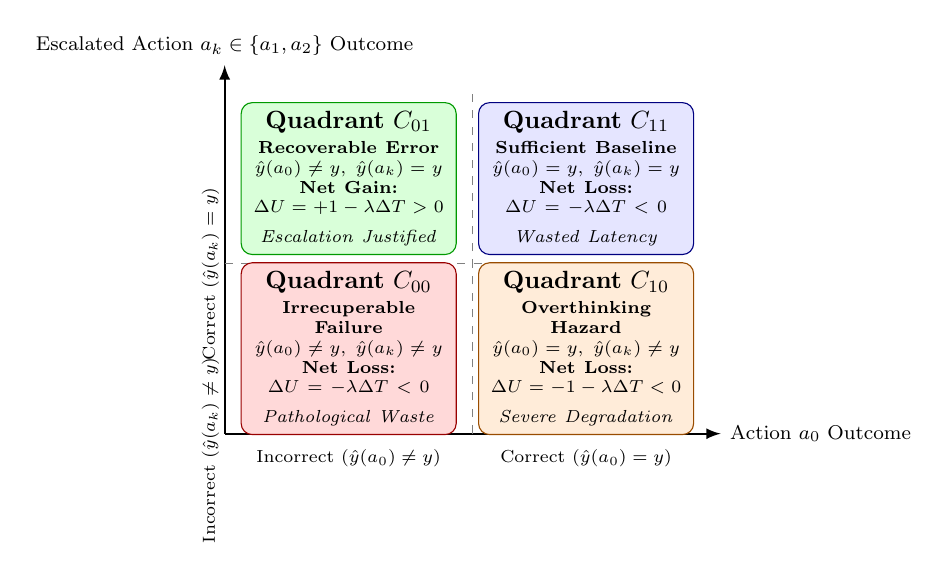
\begin{tikzpicture}[scale=0.9, every node/.style={transform shape}]
    % Grid
    \draw[thick, -latex] (0,0) -- (7,0) node[right, font=\footnotesize] {Action $a_0$ Outcome};
    \draw[thick, -latex] (0,0) -- (0,5.2) node[above, font=\footnotesize] {Escalated Action $a_k \in \{a_1, a_2\}$ Outcome};
    
    % Dividing lines
    \draw[dashed, gray] (3.5,0) -- (3.5,4.8);
    \draw[dashed, gray] (0,2.4) -- (6.5,2.4);
    
    % Quadrants
    % Top Left: C01 Recoverable
    \node[fill=green!15, rounded corners, draw=green!60!black, text width=2.8cm, text centered, minimum height=1.9cm] at (1.75, 3.6) {
        \textbf{Quadrant $C_{01}$}\\[2pt]
        \scriptsize \textbf{Recoverable Error}\\
        $\hat{y}(a_0) \neq y, \; \hat{y}(a_k) = y$\\
        \textbf{Net Gain:}\\
        $\Delta U = +1 - \lambda \Delta T > 0$\\
        \emph{Escalation Justified}
    };
    
    % Top Right: C11 Both Correct
    \node[fill=blue!10, rounded corners, draw=blue!50!black, text width=2.8cm, text centered, minimum height=1.9cm] at (5.1, 3.6) {
        \textbf{Quadrant $C_{11}$}\\[2pt]
        \scriptsize \textbf{Sufficient Baseline}\\
        $\hat{y}(a_0) = y, \; \hat{y}(a_k) = y$\\
        \textbf{Net Loss:}\\
        $\Delta U = -\lambda \Delta T < 0$\\
        \emph{Wasted Latency}
    };
    
    % Bottom Left: C00 Irrecuperable
    \node[fill=red!15, rounded corners, draw=red!60!black, text width=2.8cm, text centered, minimum height=1.9cm] at (1.75, 1.2) {
        \textbf{Quadrant $C_{00}$}\\[2pt]
        \scriptsize \textbf{Irrecuperable Failure}\\
        $\hat{y}(a_0) \neq y, \; \hat{y}(a_k) \neq y$\\
        \textbf{Net Loss:}\\
        $\Delta U = -\lambda \Delta T < 0$\\
        \emph{Pathological Waste}
    };
    
    % Bottom Right: C10 Overthinking
    \node[fill=orange!15, rounded corners, draw=orange!60!black, text width=2.8cm, text centered, minimum height=1.9cm] at (5.1, 1.2) {
        \textbf{Quadrant $C_{10}$}\\[2pt]
        \scriptsize \textbf{Overthinking Hazard}\\
        $\hat{y}(a_0) = y, \; \hat{y}(a_k) \neq y$\\
        \textbf{Net Loss:}\\
        $\Delta U = -1 - \lambda \Delta T < 0$\\
        \emph{Severe Degradation}
    };
    
    % Labels on axes
    \node[below, font=\scriptsize] at (1.75, -0.1) {Incorrect ($\hat{y}(a_0) \neq y$)};
    \node[below, font=\scriptsize] at (5.1, -0.1) {Correct ($\hat{y}(a_0) = y$)};
    \node[left, font=\scriptsize, rotate=90] at (-0.2, 1.2) {Incorrect ($\hat{y}(a_k) \neq y$)};
    \node[left, font=\scriptsize, rotate=90] at (-0.2, 3.6) {Correct ($\hat{y}(a_k) = y$)};
\end{tikzpicture}%
}
\caption{Taxonomy of joint classification events between baseline $a_0$ and complex action $a_k \in \{a_1, a_2\}$. Escalate decisions are profitable \emph{only} in Quadrant $C_{01}$ (recoverable errors). Confidence thresholds cannot distinguish $C_{01}$ from $C_{00}$, squandering budget in deep-noise regimes.}
\label{fig:recoverability_quadrants}
\end{figure}

\begin{itemize}
    \item \textbf{Quadrant $C_{11}$ (Both Correct):} Both $a_0$ and $a_k$ yield the correct class. Escalating to $a_k$ yields zero accuracy improvement while incurring latency penalty $\Delta T = T_{\mathrm{total}}(a_k) - T_{\mathrm{total}}(a_0)$, resulting in a net utility loss $\Delta U = -\lambda \Delta T < 0$.
    
    \item \textbf{Quadrant $C_{01}$ (Recoverable Error):} Baseline $a_0$ fails ($\hat{y}(a_0) \neq y$) but $a_k$ succeeds ($\hat{y}(a_k) = y$). Escalation recovers the correct class, generating a net gain $\Delta U = +1 - \lambda \Delta T > 0$ provided $\lambda \Delta T < 1$.
    
    \item \textbf{Quadrant $C_{00}$ (Irrecuperable Error):} Both $a_0$ and $a_k$ fail due to extreme channel degradation (e.g., $\mathrm{SNR} \le -15\,\mathrm{dB}$ or deep spectral nulls below the Shannon classification limit). Escalation produces no accuracy improvement and incurs full latency penalty: $\Delta U = -\lambda \Delta T < 0$.
    
    \item \textbf{Quadrant $C_{10}$ (Overthinking / Degradation):} Baseline $a_0$ succeeds, but $a_k$ misclassifies due to representation sensitivity or overfitting. Escalation incurs a catastrophic penalty $\Delta U = -1 - \lambda \Delta T \ll 0$.
\end{itemize}

Under severe noise ($C_{00}$), classifier $a_0$ exhibits near-zero margin and maximal entropy, exactly mirroring its behavior on recoverable edge cases ($C_{01}$). Consequently, any scalar threshold $\tau_{\mathrm{conf}}$ triggers escalation on both $C_{01}$ and $C_{00}$, expending massive acquisition and compute budgets on hopelessly corrupted signals. In contrast, maximizing expected net utility \eqref{eq:bayes_optimal_policy} directly estimates the counterfactual recovery probability:
\begin{align}
    \Delta \hat{U}_{k \mid 0}(\mathbf{g}) &= \hat{\mathbb{P}}(C_{01}^{(k)} \mid \mathbf{g}) - \hat{\mathbb{P}}(C_{10}^{(k)} \mid \mathbf{g}) \nonumber \\
    &\quad - \lambda [T_{\mathrm{total}}(a_k) - T_{\mathrm{total}}(a_0)],
    \label{eq:delta_utility}
\end{align}
which is positive \emph{if and only if} the likelihood of recovery exceeds the cost-adjusted risk of unrecoverable or degraded execution.

\subsubsection{Physical Bifurcation of Recoverable Errors}
Furthermore, the proposed tripartite action space admits a physical bifurcation of recoverable errors:
\begin{equation}
    C_{01} = C_{01}^{(a_1)} \cup C_{01}^{(a_2)}.
    \label{eq:bifurcation}
\end{equation}
When distortion arises from finite-sample moment estimation variance in stationary moderate-SNR channels, high-order statistics stabilize over longer durations; such errors belong to $C_{01}^{(a_1)}$ and are resolved by extending observation to $N_1 = 512$ ($a_1$). Conversely, when errors are caused by multipath frequency selectivity, residual carrier offset, or high-order constellation crowding ($16\mathrm{QAM} / 64\mathrm{QAM}$), expanding $N$ with scalar moment classifiers provides negligible gain. Such errors belong to $C_{01}^{(a_2)}$ and require the polyphase attention and multi-harmonic spectral transformations of $a_2$. The policy must therefore discern not merely whether to escalate, but \emph{which physical resource} (observation vs. computation) recovers the transmission.

% -------------------------------------------------------------------------
\subsection{Fast LBAP Selector Architecture and Formulation}
\label{subsec:lbap_architecture}

To evaluate \eqref{eq:bayes_optimal_policy} within real-time budgets ($<0.05\,\mathrm{ms}$), we design the \emph{Fast LBAP Selector} as a hybrid architecture coupling a convex Ridge regularizer with an ultra-compact two-layer Multi-Layer Perceptron (MLP), implemented in vectorized C-contiguous NumPy array routines.

\subsubsection{Gating Representation Vector $\mathbf{g} \in \mathbb{R}^{74}$}
The gating vector $\mathbf{g} = [\mathbf{f}_{256}^T, \mathbf{s}^T, m, \hat{p}_0, H]^T \in \mathbb{R}^{74}$ encapsulates:
\begin{enumerate}
    \item \textbf{Statistical and Spectral Features ($\mathbf{f}_{256} \in \mathbb{R}^{65}$):} Sample cumulants ($\hat{C}_{20}, \hat{C}_{40}, \hat{C}_{42}, \hat{C}_{60}, \hat{C}_{63}$), normalized envelope central moments up to 6th order, cyclic phase projections $R_k = |\mathbb{E}[e^{j k \arg(r[n])}]|$ for $k \in \{1, 2, 4, 8\}$, spectral flatness, and spectral entropy.
    \item \textbf{SVM Decision Projections ($\mathbf{s} \in \mathbb{R}^6$):} The signed uncalibrated distances $s_c(\mathbf{f}_{256})$ to the decision hyperplanes for all six classes $c \in \mathcal{C}$ generated by $\mathrm{SVM}_{256}$.
    \item \textbf{Top-Two Margin ($m \in \mathbb{R}$):} The difference between the highest and second-highest decision scores: $m = s_{(1)} - s_{(2)} \ge 0$.
    \item \textbf{Calibrated Posterior Confidence ($\hat{p}_0 \in [0, 1]$):} The logistic-calibrated probability of baseline correctness $\hat{p}_0 = \sigma(\beta_1 m + \beta_0)$ fitted strictly on validation data (Section~\ref{subsec:calibration}).
    \item \textbf{Normalized Decision Entropy ($H \in [0, 1]$):} Evaluating ambiguity across the class distribution:
    \begin{equation}
        H = -\frac{1}{\ln 6} \sum_{c=1}^6 \tilde{p}_c \ln(\tilde{p}_c + \epsilon), \quad \tilde{\mathbf{p}} = \mathrm{softmax}(\mathbf{s}).
        \label{eq:decision_entropy}
    \end{equation}
\end{enumerate}

\subsubsection{Hybrid Ridge--MLP Estimator}
Input features are standardized using frozen parameters computed on the training set:
\begin{equation}
    \tilde{\mathbf{g}} = \mathrm{clip}\left( \frac{\mathbf{g} - \boldsymbol{\mu}_{\mathbf{g}}}{\boldsymbol{\sigma}_{\mathbf{g}} + \epsilon_{\mathrm{scale}}}, -10.0, 10.0 \right) \in \mathbb{R}^{74}.
    \label{eq:input_standardization}
\end{equation}

The utility predictor decomposes into two complementary functional pathways:
\begin{enumerate}
    \item \textbf{Linear Ridge Pathway (Global Regularized Baseline):}
    \begin{equation}
        \mathbf{u}_{\mathrm{lin}}(\mathbf{g}) = \tilde{\mathbf{g}} \mathbf{W}_{\mathrm{lin}} + \mathbf{b}_{\mathrm{lin}},
        \label{eq:ridge_path}
    \end{equation}
    where $\mathbf{W}_{\mathrm{lin}} \in \mathbb{R}^{74 \times 3}$ and $\mathbf{b}_{\mathrm{lin}} \in \mathbb{R}^3$ are solved in closed form via Tikhonov regularization with parameter $\gamma_{\mathrm{ridge}} = 40.0$:
    \begin{equation}
        \mathbf{W}_{\mathrm{lin}} = (\tilde{\mathbf{G}}^T \tilde{\mathbf{G}} + \gamma_{\mathrm{ridge}} \mathbf{I})^{-1} \tilde{\mathbf{G}}^T (\mathbf{Y}_{\mathrm{util}} - \bar{\mathbf{Y}}_{\mathrm{util}}),
        \label{eq:ridge_closed_form}
    \end{equation}
    guaranteeing bounded variance and numerical stability across collinear cumulant features.
    
    \item \textbf{Non-Linear MLP Pathway (Local Interaction Modeler):}
    \begin{align}
        \mathbf{h} &= \max(0, \tilde{\mathbf{g}} \mathbf{W}_1 + \mathbf{b}_1), \quad \mathbf{h} \in \mathbb{R}^{d_h}, \label{eq:mlp_hidden} \\
        \mathbf{u}_{\mathrm{mlp}}(\mathbf{g}) &= \mathbf{h} \mathbf{W}_2 + \mathbf{b}_2, \quad \mathbf{u}_{\mathrm{mlp}} \in \mathbb{R}^3, \label{eq:mlp_output}
    \end{align}
    with hidden dimension $d_h = 64$. The MLP parameters are trained to minimize the robust Huber (Smooth $L_1$) loss against ground-truth counterfactual utilities:
    \begin{equation}
        \mathcal{L}_{\mathrm{Huber}}(\mathbf{u}, \mathbf{y}) = \sum_{a=0}^2 \begin{cases} 
            0.5 (u_a - y_a)^2, & |u_a - y_a| \le 1, \\
            |u_a - y_a| - 0.5, & \text{otherwise},
        \end{cases}
        \label{eq:huber_loss}
    \end{equation}
    optimized via AdamW (learning rate $\eta = 3\times 10^{-3}$, weight decay $10^{-3}$, $400$ epochs).
\end{enumerate}

\subsubsection{Convex Ensembling and Action Selection}
The final predicted utility vector $\hat{\mathbf{u}}(\mathbf{g}) = [\hat{u}_0, \hat{u}_1, \hat{u}_2]^T$ blends both pathways:
\begin{equation}
    \hat{\mathbf{u}}(\mathbf{g}) = \alpha^* \mathbf{u}_{\mathrm{mlp}}(\mathbf{g}) + (1 - \alpha^*) \mathbf{u}_{\mathrm{lin}}(\mathbf{g}),
    \label{eq:blended_utility}
\end{equation}
where the ensembling weight $\alpha^* \in \{0.0, 0.25, 0.50, 0.75, 1.0\}$ is tuned on an independent validation set $\mathcal{V}_{\mathrm{select}}$ to maximize realized classification utility. The policy selects the action that maximizes predicted net utility over the allowed action subset $\mathcal{A}_{\mathrm{allowed}} \subseteq \mathcal{A}$:
\begin{equation}
    a^*(\mathbf{g}) = \arg\max_{a \in \mathcal{A}_{\mathrm{allowed}}} \; \hat{u}_a(\mathbf{g}).
    \label{eq:final_action_choice}
\end{equation}

When restricted to $\mathcal{A}_{\mathrm{allowed}} = \{a_0, a_1\}$, the model reduces to pure adaptive acquisition (Fewer-Sample style); when restricted to $\mathcal{A}_{\mathrm{allowed}} = \{a_0, a_2\}$, it instantiates early-exit computational escalation (BEACON style). The unrestricted set $\mathcal{A}_{\mathrm{allowed}} = \{a_0, a_1, a_2\}$ realizes joint observation-computation optimization.

% -------------------------------------------------------------------------
\subsection{Rigorous Probabilistic Calibration and Temperature Scaling}
\label{subsec:calibration}

In safety-critical wireless systems, decision policies must not rely on uncalibrated heuristic scores. Raw margin scores from SVMs and uncalibrated softmax logits from deep neural networks suffer from severe overconfidence in low-SNR and out-of-distribution (OOD) regimes \cite{yang2026uncertainty}. To prevent policy distortion, we establish rigorous calibration protocols on an isolated calibration partition $\mathcal{V}_{\mathrm{cal}}$ ($1200$ balanced signals) strictly disjoint from both the policy-selection partition $\mathcal{V}_{\mathrm{select}}$ ($1200$ signals) and the test splits.

\subsubsection{Margin-Based Platt Calibration for Baseline $a_0$}
For $\mathrm{SVM}_{256}$, class assignment is determined by $\hat{y}(a_0) = \arg\max_{c \in \mathcal{C}} s_c$. The probability that this assignment is correct is modeled via a univariate logistic sigmoid over the margin $m = s_{(1)} - s_{(2)}$:
\begin{equation}
    \hat{P}(Y = \hat{y}(a_0) \mid m) = \sigma(\beta_1 m + \beta_0) = \frac{1}{1 + e^{-(\beta_1 m + \beta_0)}},
    \label{eq:platt_margin}
\end{equation}
where parameters $\boldsymbol{\beta} = [\beta_1, \beta_0]^T$ are fitted by minimizing the binary cross-entropy loss over $\mathcal{V}_{\mathrm{cal}}$ with $L_2$ regularization:
\begin{align}
    \min_{\boldsymbol{\beta}} \; -\sum_{i \in \mathcal{V}_{\mathrm{cal}}} \Big[ &z_i \ln \sigma(\beta_1 m_i + \beta_0) \nonumber \\
    &+ (1 - z_i) \ln\big(1 - \sigma(\beta_1 m_i + \beta_0)\big) \Big],
    \label{eq:logistic_cal_loss}
\end{align}
where $z_i = \mathbb{I}(\hat{y}^{(i)}(a_0) = y^{(i)})$. This single calibrated probability $\hat{p}_0$ is injected directly into dimension $73$ of the gating vector $\mathbf{g}$.

\subsubsection{Temperature Scaling for Deep Expert $a_2$}
For $\mathrm{MultiDomainAMCNet}$ ($a_2$), raw forward inference outputs unnormalized logits $\mathbf{z}(\mathbf{r}_{256}) \in \mathbb{R}^6$. Applying a naive softmax $p_k = e^{z_k} / \sum_j e^{z_j}$ produces miscalibrated confidence scores under channel mismatch. We apply parametric Temperature Scaling \cite{yang2026uncertainty}, modifying logits by a single strictly positive scalar temperature $T > 0$:
\begin{equation}
    \hat{p}_k(\mathbf{r}_{256}; T) = \frac{\exp(z_k / T)}{\sum_{j=1}^6 \exp(z_j / T)}, \quad \forall k \in \{1, \dots, 6\}.
    \label{eq:temp_scaling}
\end{equation}
The optimal temperature $T^*$ is identified by minimizing the multiclass Negative Log-Likelihood (NLL) over the held-out calibration set $\mathcal{V}_{\mathrm{cal}}$:
\begin{equation}
    T^* = \arg\min_{T > 0} \; -\sum_{i \in \mathcal{V}_{\mathrm{cal}}} \sum_{c=1}^6 \mathbb{I}(y^{(i)} = c) \ln \hat{p}_c(\mathbf{r}_{256}^{(i)}; T),
    \label{eq:temp_nll_opt}
\end{equation}
solved via the quasi-Newton L-BFGS optimizer. Crucially, because the transformation $\mathbf{z} / T$ is strictly monotonic for any $T > 0$, temperature scaling preserves the classification output $\arg\max_k z_k$ and the top-1 accuracy identically, while calibrating the output probabilities to align with empirical accuracy.

Calibration quality for top-1 confidence reliability is quantified via the Expected Calibration Error ($\mathrm{ECE}_{10}$) over $K=10$ uniform equal-width bins in $[0, 1]$:
\begin{equation}
    \mathrm{ECE}_{10} = \sum_{b=1}^{10} \frac{|B_b|}{N_{\mathrm{val}}} \left| \mathrm{acc}(B_b) - \mathrm{conf}(B_b) \right|,
    \label{eq:ece_def}
\end{equation}
together with binary top-1 correctness Brier score $\mathrm{BS}_{\mathrm{bin}} = \frac{1}{N} \sum_{i=1}^N (\hat{p}_{i,\max} - z_i)^2$ and binary Negative Log-Likelihood $\mathrm{NLL}_{\mathrm{bin}} = -\frac{1}{N}\sum_{i=1}^N [z_i \ln \hat{p}_{i,\max} + (1 - z_i)\ln(1 - \hat{p}_{i,\max})]$, where $z_i = \mathbb{I}(\hat{y}_i = y_i)$ and $\hat{p}_{i,\max} = \max_c \hat{p}_{ic}$ (allowing unified scalar reliability comparison across both the binary Platt margin of $a_0$ and the maximum calibrated probability of $a_2$). Note that $T^*$ is nevertheless optimized via multiclass NLL~\eqref{eq:temp_nll_opt}. As quantified in Section~\ref{sec:results_discussion}, post-hoc calibration aligns the in-distribution confidence scores of both the baseline SVM and the deep expert with empirical accuracy, while revealing overconfidence degradation under severe OOD shift.

% -------------------------------------------------------------------------
\subsection{Pareto Optimality across Latency Regimes and Sampling Frequencies}
\label{subsec:pareto_formulation}

A fundamental advantage of the proposed net utility formulation is its adaptability across heterogeneous operational environments. By varying the latency cost parameter $\lambda$ and analyzing system behavior across different front-end ADC sampling frequencies $f_s$, the Fast LBAP selector defines an optimal Pareto frontier balancing classification risk $R(\pi) = 1 - \mathrm{Acc}(\pi)$ against total reception latency $T_{\mathrm{total}}(\pi)$.

\begin{figure}[t]
\centering
\resizebox{\columnwidth}{!}{%
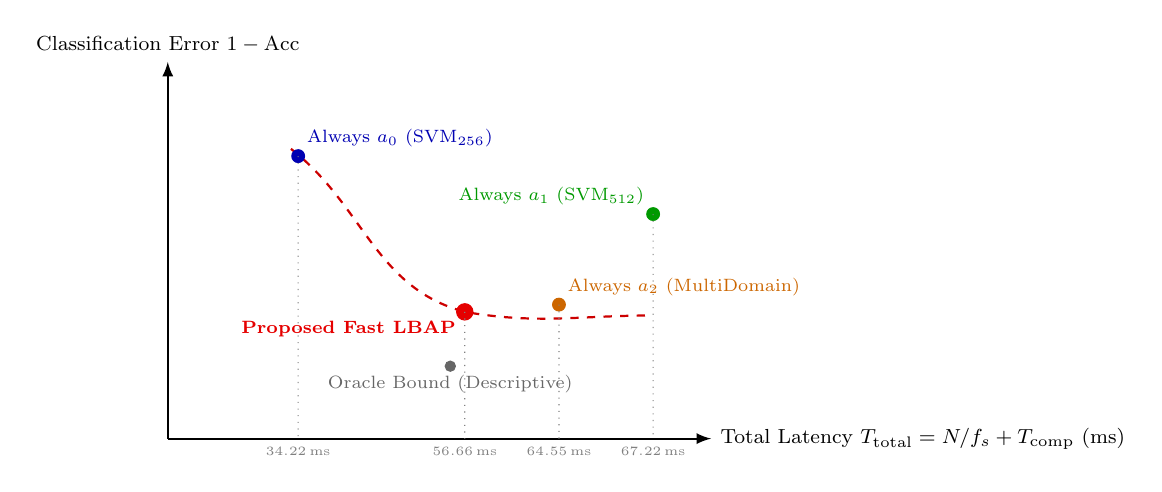
\begin{tikzpicture}[scale=0.92, every node/.style={transform shape}]
    % Axes
    \draw[thick, -latex] (0,0) -- (7.5,0) node[right, font=\footnotesize] {Total Latency $T_{\mathrm{total}} = N/f_s + T_{\mathrm{comp}}$ (ms)};
    \draw[thick, -latex] (0,0) -- (0,5.2) node[above, font=\footnotesize] {Classification Error $1 - \mathrm{Acc}$};

    % Baselines
    \coordinate (A0) at (1.8, 3.9);
    \coordinate (A1) at (6.7, 3.1);
    \coordinate (A2) at (5.4, 1.85);
    \coordinate (LBAP_opt) at (4.1, 1.75);
    \coordinate (Oracle) at (3.9, 1.0);

    % Pareto curve
    \draw[dashed, red!80!black, thick] (1.7, 4.0) to[out=-38, in=165] (4.1, 1.75) to[out=-10, in=180] (6.7, 1.7);

    % Points
    \filldraw[blue!70!black] (A0) circle (2.5pt) node[above right, font=\scriptsize] {Always $a_0$ ($\mathrm{SVM}_{256}$)};
    \filldraw[green!60!black] (A1) circle (2.5pt) node[above left, font=\scriptsize] {Always $a_1$ ($\mathrm{SVM}_{512}$)};
    \filldraw[orange!80!black] (A2) circle (2.5pt) node[above right, font=\scriptsize] {Always $a_2$ (MultiDomain)};
    \filldraw[red!90!black] (LBAP_opt) circle (3.2pt) node[below left, font=\scriptsize\bfseries] {Proposed Fast LBAP};
    \filldraw[gray!80!black] (Oracle) circle (2pt) node[below, font=\scriptsize] {Oracle Bound (Descriptive)};

    % Grid lines
    \draw[dotted, gray] (A0) -- (1.8,0) node[below, font=\tiny] {$34.22\,\mathrm{ms}$};
    \draw[dotted, gray] (LBAP_opt) -- (4.1,0) node[below, font=\tiny] {$56.66\,\mathrm{ms}$};
    \draw[dotted, gray] (A2) -- (5.4,0) node[below, font=\tiny] {$64.55\,\mathrm{ms}$};
    \draw[dotted, gray] (A1) -- (6.7,0) node[below, font=\tiny] {$67.22\,\mathrm{ms}$};
\end{tikzpicture}%
}
\caption{Conceptual Risk--Latency Pareto frontier at $f_s = 8\,\mathrm{kHz}$ using synced full-route latency profiling (\texttt{N3.3}). At low sampling rates, the physical waiting penalty of $a_1$ ($+32\,\mathrm{ms}$) makes standalone $a_1$ ($67.22\,\mathrm{ms}$) slower than standalone $a_2$ ($64.55\,\mathrm{ms}$); deployable Fast LBAP routes across $\{a_0,a_1,a_2\}$ to achieve lower mean latency ($56.66\,\mathrm{ms}$) and higher utility ($0.4379$) than standalone $a_2$ ($0.4190$).}
\label{fig:pareto_conceptual}
\end{figure}

\subsubsection{Parametric Sensitivity to Trade-Off Coefficient $\lambda$}
The parameter $\lambda \ge 0$ represents the exchange rate between classification accuracy and reception delay:
\begin{itemize}
    \item \textbf{Accuracy-Centric Regime ($\lambda \to 0$):} Latency is unpenalized. The policy collapses to an accuracy oracle, selecting $\arg\max_{a \in \mathcal{A}} \mathbb{P}(\hat{y}(a) = y \mid \mathbf{g})$. Difficult frames are routed aggressively to the most accurate models ($a_2$ or $a_1$).
    \item \textbf{Latency-Constrained Regime ($\lambda \ge 0.005\,\mathrm{ms}^{-1}$):} An additional $32\,\mathrm{ms}$ acquisition delay penalizes net utility by $\Delta U = -0.160$. Under high latency pressure, the policy restricts escalation to high-recoverability prefixes and shifts substantially back toward immediate $a_0$ termination.
    \item \textbf{Balanced Operational Regime ($\lambda = 0.0015\,\mathrm{ms}^{-1}$):} Our nominal operating point values $10\,\mathrm{ms}$ of reception delay at $0.015$ accuracy points ($32\,\mathrm{ms}$ at $0.048$ points), balancing neural recovery against both acquisition wait ($a_1$) and single-sample inference time ($a_2$). Under this nominal trade-off with full-route synced costs, Fast LBAP improves net utility over all fixed standalone baselines in-distribution while remaining faster on average than either standalone $a_1$ or standalone $a_2$.
\end{itemize}

\subsubsection{Asymptotic Inversion with Sampling Rate $f_s$}
The relative economic advantage between action $a_1$ (more observation) and action $a_2$ (more computation) is an explicit function of the ADC sampling rate $f_s$:
\begin{align}
    \lim_{f_s \to \infty} T_{\mathrm{acq}}(a) &= 0, \quad \forall a \in \mathcal{A}, \label{eq:limit_fs_inf} \\
    \lim_{f_s \to 0} \frac{T_{\mathrm{acq}}(a_1)}{T_{\mathrm{comp}}(a_2)} &= \infty. \label{eq:limit_fs_zero}
\end{align}

In low-rate sensor and IoT networks ($f_s \approx 8\,\mathrm{kHz}$, symbol rate $R_s = 1000\,\mathrm{Bd}$), physical acquisition dominates: waiting for $256$ additional samples adds $T_{\mathrm{acq}}(a_1) - T_{\mathrm{acq}}(a_0) = 32.0\,\mathrm{ms}$ ($67.22\,\mathrm{ms}$ synced total for standalone $a_1$), whereas deep neural inference requires $T_{\mathrm{base}, 2} = 32.55\,\mathrm{ms}$ ($64.55\,\mathrm{ms}$ synced total for standalone $a_2$). In this narrowband regime, computational escalation ($a_2$) on the short $256$-sample prefix remains competitive in wall-clock delay and far more accurate in mid-SNR than extending $a_1$.

Conversely, in wideband software-defined radios and cellular transceivers ($f_s \ge 1\,\mathrm{MHz}$), physical acquisition time collapses ($T_{\mathrm{acq}}(a_1) = 512 / 10^6 = 0.512\,\mathrm{ms}$). Here, acquisition latency is negligible compared to computation, and the trade-off inverts: acquiring additional physical symbols ($a_1$) becomes virtually free, whereas arithmetic complexity ($a_2$) becomes the primary latency bottleneck. As validated by the two-dimensional Pareto sweeps in Section~\ref{sec:results_discussion}, the Fast LBAP policy autonomously adapts its action distribution across orders of magnitude in $f_s$, demonstrating true universal applicability across heterogeneous hardware constraints.
